
%\documentclass[letterpaper,english]{article}

\documentclass[letterpaper,twocolumn,english]{article}
\usepackage[T1]{fontenc}
\usepackage[latin1]{inputenc}
\usepackage{graphicx}

\usepackage{geometry}
\geometry{verbose,letterpaper,tmargin=1in,bmargin=1in,lmargin=0.75in,rmargin=0.75in}

\makeatletter

\usepackage{babel}

\begin{document}

\title{LLADD Outline }


\author{Russell Sears \and ... \and Eric Brewer}

\maketitle



\subsection*{Abstract}

{\em The sections marked @todo or bolded still need to be written, and graphs need to be produced.  Also, I would like to add a ``cheat-sheet'' style reference of an idealized version of LLADD's API.}

Existing transactional systems are designed to handle specific
workloads well.  Unfortunately, these implementations are generally
monolithic, and do not generalize to other applications or classes of
problems.  As a result, many systems are forced to ``work around'' the
data models provided by a transactional storage layer. Manifestations
of this problem include ``impedance mismatch'' in the database world,
and the poor fit of existing transactional storage management system
to hierarchical or semi-structured data types such as XML or
scientific data.  This work proposes a novel set of abstractions for
transactional storage systems and generalizes an existing
transactional storage algorithm to provide an implementation of these
primatives.  Due to the extensibility of our architecutre, the
implementation is competitive with existing systems on conventional
workloads and outperforms existing systems on specialized
workloads.  Finally, we discuss characteristics of this new
architecture which provide opportunities for novel classes of
optimizations and enhanced usability for application developers.

% todo/rcs Need to talk about collection api stuff / generalization of ARIES / new approach to application development

%Although many systems provide transactionally consistent data
%management, existing implementations are generally monolithic and tied
%to a higher-level DBMS, limiting the scope of their usefulness to a
%single application or a specific type of problem. As a result, many
%systems are forced to ``work around'' the data models provided by a
%transactional storage layer. Manifestations of this problem include
%``impedance mismatch'' in the database world and the limited number of
%data models provided by existing libraries such as Berkeley DB. In
%this paper, we describe a light-weight, easily extensible library,
%LLADD, that allows application developers to develop scalable and
%transactional application-specific data structures. We demonstrate
%that LLADD is simpler than prior systems, is very flexible and
%performs favorably in a number of micro-benchmarks. We also describe,
%in simple and concrete terms, the issues inherent in the design and
%implementation of robust, scalable transactional data structures. In
%addition to the source code, we have also made a comprehensive suite
%of unit-tests, API documentation, and debugging mechanisms publicly
%available.%
%\footnote{http://lladd.sourceforge.net/%
%}

\section{Introduction}

\begin{enumerate}

% rcs: The original intro is left intact in the other file; it would be too hard to merge right now.

  % This paragraph is a too narrow; the original was too vague 
  \item {\bf Current transactional systems handle conventional workloads
  well, but object persistence mechanisms are a mess, as are
  {}``version oriented'' data stores requiring large, efficient atomic
  updates.}

  \item {\bf {}``Impedance mismatch'' is a term that refers to a mismatch
  between the data model provided by the data store and the data model
  required by the application. A significant percentage of software
  development effort is related to dealing with this problem. Related
  problems that have had less treatment in the literature involve
  mismatches between other performance-critical and labor intensive
  programming primitives such as concurrency models, error handling
  techniques and application development patterns.}
% rcs: see ##1## in other file for more examples
  \item {\bf Past trends in the Database community have been driven by
  demand for tools that allow extremely specialized (but commercially
  important!)  types of software to be developed quickly and
  inexpensively. {[}System R, OODBMS, benchmarks, streaming databases,
  etc{]} This has led to the development of large, monolithic database
  severs that perform well under many circumstances, but that are not
  nearly as flexible as modern programming languages or typical
  in-memory data structure libraries {[}Java Collections,
  STL{]}. Historically, programming language and software library
  development has focused upon the production of a wide array of
  composable general purpose tools, allowing the application developer
  to pick algorithms and data structures that are most appropriate for
  the problem at hand.}

  \item {\bf In the past, modular database and transactional storage
  implementations have hidden the complexities of page layout,
  synchronization, locking, and data structure design under relatively
  narrow interfaces, since transactional storage algorithms'
  interdependencies and requirements are notoriously complicated.}

%Not implementing ARIES any more!


  \item {\bf With these trends in mind, we have implemented a modular
  version of ARIES that makes as few assumptions as possible about
  application data structures or workload. Where such assumptions are
  inevitable, we have produced narrow APIs that allow the application
  developer to plug in alternative implementations of the modules that
  comprise our ARIES implementation. Rather than hiding the underlying
  complexity of the library from developers, we have produced narrow,
  simple API's and a set of invariants that must be maintained in
  order to ensure transactional consistency, allowing application
  developers to produce high-performance extensions with only a little
  effort.}

\end{enumerate}
\section{Prior work}

\begin{enumerate}

  \item{\bf Databases' Relational model leads to performance /
  representation problems.}

On the database side of things, relational databases excel in areas
where performance is important, but where the consistency and
durability of the data are crucial.  Often, databases significantly
outlive the software that uses them, and must be able to cope with
changes in business practices, system architectures,
etc.~\cite{relational}

Databases are designed for circumstances where development time may
dominate cost, many users must share access to the same data, and
where security, scalability, and a host of other concerns are
important.  In many, if not most circumstances these issues are less
important, or even irrelevant.  Therefore, applying a database in
these situations is likely overkill, which may partially explain the
popularity of MySQL~\cite{mysql}, which allows some of these
constraints to be relaxed at the discretion of a developer or end
user.

  \item{\bf OODBMS / XML database systems provide models tied closely to PL
  or hierarchical formats, but, like the relational model, these
  models are extremely general, and might be inappropriate for
  applications with stringent performance demands, or that use these
  models in a way that cannot be supported well with the database
  system's underlying data structures.}

Object-oriented databases are more focused on facilitating the
development of complex applications that require reliable storage and
may take advantage of less-flexible, more efficient data models, as
they often only interact with a single application, or a handful of
variants of that application.~\cite{lamb}

  \item{\bf Berkeley DB provides a lower level interface, increasing
  performance, and providing efficient tree and hash based data
  structures, but hides the details of storage management and the
  primitives provided by its transactional layer from
  developers. Again, only a handful of data formats are made available
  to the developer.}

%rcs: The inflexibility of databases has not gone unnoticed ... or something like that.

Still, there are many applications where MySQL is too inflexible.  In
order to serve these applications, a host of software solutions have
been devised.  Some are extremely complex, such as semantic file
systems, where the file system understands the contents of the files
that it contains, and is able to provide services such as rapid
search, or file-type specific operations such as thumb-nailing,
automatic content updates, and so on.  Others are simpler, such as
Berkeley~DB,~\cite{berkeleyDB, bdb} which provides transactional
storage of data in unindexed form, or in indexed form using a hash
table or tree.  LRVM is a version of malloc() that provides
transactional memory, and is similar to an object-oriented database
but is much lighter weight, and more flexible~\cite{lrvm}.

  \item {\bf Incredibly scalable, simple servers CHT's, google fs?, ...}

Finally, some applications require incredibly simple, but extremely
scalable storage mechanisms.  Cluster hash tables are a good example
of the type of system that serves these applications well, due to
their relative simplicity, and extremely good scalability
characteristics.  Depending on the fault model on which a cluster hash
table is implemented, it is quite plausible that key portions of the
transactional mechanism, such as forcing log entries to disk, will be
replaced with other durability schemes, such as in-memory replication
across many nodes, or multiplexing log entries across multiple
systems.  This level of flexibility would be difficult to retrofit
into existing transactional applications, but is often important in
the environments in which these applications are deployed.


  \item {\bf Implementations of ARIES and other transactional storage
  mechanisms include many of the useful primitives described below,
  but prior implementations either deny application developers access
  to these primitives {[}??{]}, or make many high-level assumptions
  about data representation and workload {[}DB Toolkit from
  Wisconsin??-need to make sure this statement is true!{]}}

\end{enumerate}

%\item {\bf 3.Architecture  }

\section{Write ahead logging overview}

This section describes how existing write ahead logging protocols
implement the four properties of transactional storage: Atomicity,
Consistency, Isolation and Durability.  LLADD provides these four
properties to applications but also allows applications to opt-out of
certain of properties as appropriate.  This can be useful for
performance reasons or to simplify the mapping between application
semantics and the storage layer.  Unlike prior work, LLADD also
exposes the primatives described below to application developers,
allowing unanticipated optimizations to be implemented and allowing
low level behavior such as recovery semantics to be customized on a
per-application basis.

The write ahead logging algorithm we use is based upon ARIES. Because
comprehensive discussions of write ahead logging protocols and ARIES
are available elsewhere,~\cite{haerder, aries} we focus upon those
details which are most important to the architecture this paper
presents.



%Instead of providing a comprehensive discussion of ARIES, we will
%focus upon those features of the algorithm that are most relevant
%to a developer attempting to add a new set of operations. Correctly
%implementing such extensions is complicated by concerns regarding
%concurrency, recovery, and the possibility that any operation may
%be rolled back at runtime.
%
%We first sketch the constraints placed upon operation implementations,
%and then describe the properties of our implementation that
%make these constraints necessary. Because comprehensive discussions of
%write ahead logging protocols and ARIES are available elsewhere,~\cite{haerder, aries} we
%only discuss those details relevant to the implementation of new
%operations in LLADD.


\subsection{Operations\label{sub:OperationProperties}}

A transaction consists of an arbitrary combination of actions, that
will be protected according to the ACID properties mentioned above.
Since transactions may be aborted, the effects of an action must be
reversible, implying that any information that is needed in order to
reverse the action must be stored for future use.  Typically, the
information necessary to redo and undo each action is stored in the
log.  We refine this concept and explicitly discuss {\em operations},
which must be atomically applicable to the page file.  For now, we
simply assume that operations do not span pages, and that pages are
atomically written to disk.  This limitation will relaxed when we
describe how to implement page-spanning operations using techniques
such as nested top actions.

\subsection{Concurrency}

We allow transactions to be interleaved, allowing concurrent access to
application data and exploiting opportunities for hardware
parallelism.  Therefore, each action must assume that the
physical data upon which it relies may contain uncommitted
information and that this information may have been produced by a
transaction that will be aborted by a crash or by the application.

% Furthermore, aborting
%and committing transactions may be interleaved, and LLADD does not
%allow cascading aborts,%
%\footnote{That is, by aborting, one transaction may not cause other transactions
%to abort. To understand why operation implementors must worry about
%this, imagine that transaction A split a node in a tree, transaction
%B added some data to the node that A just created, and then A aborted.
%When A was undone, what would become of the data that B inserted?%
%} so 

Therefore, in order to implement an operation we must also implement
synchronization mechanisms that isolate the effects of transactions
from each other.  We use the term {\em latching} to refer to
synchronization mechanisms that protect the physical consistency of
LLADD's internal data structures and the data store.  We say {\em
locking} when we refer to mechanisms that provide some level of
isolation between transactions.  

LLADD operations that allow concurrent requests must provide a
latching implementation that is guaranteed not to deadlock.  These
implementations need not ensure consistency of application data.
Instead, they must maintain the consistency of any underlying data
structures.

Due to the variety of locking systems available, and their interaction
with application workload,~\cite{multipleGenericLocking} we leave it
to the application to decide what sort of transaction isolation is
appropriate.  LLADD provides a simple page level lock manager that
performs deadlock detection, although we expect many applications to
make use of deadlock avoidance schemes, which are prevalent in
multithreaded application development.

For example, would be relatively easy to build a strict two-phase
locking lock
manager~\cite{hierarcicalLocking,hierarchicalLockingOnAriesExample} on
top of LLADD.  Such a lock manager would provide isolation guarantees
for all applications that make use of it.  However, applications that
make use of such a lock manager must check for (and recover from)
deadlocked transactions that have been aborted by the lock manager,
complicating application code.

Many applications do not require such a general scheme.  For instance,
an IMAP server could employ a simple lock-per-folder approach and use
lock ordering techniques to avoid the possiblity of deadlock.  This
would avoid the complexity of dealing with transactions that abort due
to deadlock, and also remove the runtime cost of aborted and retried
transactions.  

Currently, LLADD provides an optional page-level lock manager.  We are
unaware of any limitations in our architecture that would prevent us
from implementing full hierarchical locking and index locking in the
future.  We will revisit this point in more detail when we describe
the sample operations that we have implemented.

%Thus, data dependencies among
%transactions are allowed, but we still must ensure the physical
%consistency of our data structures, such as operations on pages or locks.

\subsection{The Log Manager}

All actions performed by a committed transaction must be
restored in the case of a crash, and all actions performed by aborting
transactions must be undone. In order for LLADD to arrange for this
to happen at recovery, operations must produce log entries that contain
all information necessary for undo and redo.

An important concept in ARIES is the ``log sequence number'' or {\em
LSN}.  An LSN is essentially a virtual timestamp that goes on every
page; it marks the last log entry that is reflected on the page and
implies that all previous log entries are also reflected.  Given the
LSN, LLADD calculates where to start playing back the log to bring the
page up to date.  The LSN is stored in the page that it refers to so
that it is always written to disk atomically with the data on the
page.

ARIES (and thus LLADD) allows pages to be {\em stolen}, i.e. written
back to disk while they still contain uncommitted data.  It is
tempting to disallow this, but to do so has serious consequences such as
a increased need for buffer memory (to hold all dirty pages). Worse,
as we allow multiple transactions to run concurrently on the same page
(but not typically the same item), it may be that a given page {\em
always} contains some uncommitted data and thus could never be written
back to disk.  To handle stolen pages, we log UNDO records that
we can use to undo the uncommitted changes in case we crash.  LLADD
ensures that the UNDO record is durable in the log before the
page is written to disk and that the page LSN reflects this log entry.

Similarly, we do not force pages out to disk every time a transaction
commits, as this limits performance.  Instead, we log REDO records
that we can use to redo the operation in case the committed version never
makes it to disk.  LLADD ensures that the REDO entry is durable in the
log before the transaction commits.  REDO entries are physical changes
to a single page (``page-oriented redo''), and thus must be redone in
order.

One unique aspect of LLADD, which is not true for ARIES, is that {\em
normal} operations use the REDO function; i.e. there is no way to
modify the page except via the REDO operation.\footnote{Actually,
operation implementations may circumvent this restriction, but doing
so complicates recovery semantics, and only should be done as a last
resort.  Currently, this is only done to implement the OASYS flush()
and update() operations described in Section~\ref{OASYS}.}  This has
the nice property that the REDO code is known to work, since even the
original update is a ``redo''.  In general, the LLADD philosophy is
that you define operations in terms of their REDO/UNDO behavior, and
then build a user friendly interface around those.

Eventually, the page makes it to disk, but the REDO entry is still
useful; we can use it to roll forward a single page from an archived
copy.  Thus one of the nice properties of LLADD, which has been
tested, is that we can handle media failures very gracefully: lost
disk blocks or even whole files can be recovered given an old version
and the log.  

\subsection{Recovery}

%In this section, we present the details of crash recovery, user-defined logging, and atomic actions that commit even if their enclosing transaction aborts.
%
%\subsubsection{ANALYSIS / REDO / UNDO}

Recovery in ARIES consists of three stages: {\em analysis}, {\em redo} and {\em undo}. 
The first, analysis, is
implemented by LLADD, but will not be discussed in this
paper. The second, redo, ensures that each redo entry in the log 
will have been applied to each page in the page file exactly once.
The third phase, undo, rolls back any transactions that were active
when the crash occurred, as though the application manually aborted
them with the {}``abort'' function call.
  
After the analysis phase, the on-disk version of the page file
is in the same state it was in when LLADD crashed. This means that
some subset of the page updates performed during normal operation
have made it to disk, and that the log contains full redo and undo
information for the version of each page present in the page file.%
\footnote{Although this discussion assumes that the entire log is present, the
ARIES algorithm supports log truncation, which allows us to discard
old portions of the log, bounding its size on disk.%
} Because we make no further assumptions regarding the order in which
pages were propagated to disk, redo must assume that any
data structures, lookup tables, etc. that span more than a single
page are in an inconsistent state. Therefore, as the redo phase re-applies
 the information in the log to the page file, it must address all pages directly. 

This implies that the redo information for each operation in the log
must contain the physical address (page number) of the information
that it modifies, and the portion of the operation executed by a single
redo log entry must only rely upon the contents of the page that the 
entry refers to. Since we assume that pages are propagated to disk
atomically, the redo phase may rely upon information contained within
a single page.

Once redo completes, we have applied some prefix of the run-time log.
Therefore, we know that the page file is in
a physically consistent state, although it contains portions of the
results of uncommitted transactions. The final stage of recovery is
the undo phase, which simply aborts all uncommitted transactions. Since
the page file is physically consistent, the transactions may be aborted
exactly as they would be during normal operation. 


\subsection{Physical, Logical and Physiological Logging.}

The above discussion avoided the use of some common terminology 
that should be presented here. {\em Physical logging } 
is the practice of logging physical (byte-level) updates
and the physical (page number) addresses to which they are applied.

{\em Physiological logging } is what LLADD recommends for its redo 
records. The physical address (page number) is stored, but the byte offset
and the actual difference are stored implicitly in the parameters
of the redo or undo function. These parameters allow the function to 
update the page in a way that preserves application semantics.
One common use for this is {\em slotted pages}, which use an on-page level of 
indirection to allow records to be rearranged within the page; instead of using the page offset, redo 
operations use a logical offset to locate the data. This allows data within
a single page to be re-arranged at runtime to produce contiguous
regions of free space. LLADD generalizes this model; for example, the parameters passed to the function may utilize application specific properties in order to be significantly smaller than the physical change made to the page.~\cite{physiological}

{\em Logical logging } can only be used for undo entries in LLADD, and
stores a logical address (the key of a hash table, for instance)
instead of a physical address. As we will see later, these operations
may affect multiple pages.  This allows the location of data in the
page file to change, even if outstanding transactions may have to roll
back changes made to that data. Clearly, for LLADD to be able to apply
logical log entries, the page file must be physically consistent,
ruling out use of logical logging for redo operations.

LLADD supports all three types of logging, and allows developers to
register new operations, which is the key to its extensibility. After
discussing LLADD's architecture, we will revisit this topic with a number of
concrete examples.


\subsection{Concurrency and Aborted Transactions}

% @todo this section is confusing.  Re-write it in light of page spanning operations, and the fact that we assumed opeartions don't span pages above.  A nested top action (or recoverable, carefully ordered operation) is simply a way of causing a page spanning operation to be applied atomically.  (And must be used in conjunction with latches...)  Note that the combination of latching and NTAs makes the implementation of a page spanning operation no harder than normal multithreaded software development.

Section~\ref{sub:OperationProperties} states that LLADD does not
allow cascading aborts, implying that operation implementors must
protect transactions from any structural changes made to data structures
by uncommitted transactions, but LLADD does not provide any mechanisms
designed for long-term locking. However, one of LLADD's goals is to
make it easy to implement custom data structures for use within safe,
multi-threaded transactions. Clearly, an additional mechanism is needed.

The solution is to allow portions of an operation to ``commit'' before
the operation returns.\footnote{We considered the use of nested top actions, which LLADD could easily
support. However, we currently use the slightly simpler (and lighter-weight)
mechanism described here. If the need arises, we will add support
for nested top actions.}
An operation's wrapper is just a normal function, and therefore may
generate multiple log entries. First, it writes an undo-only entry
to the log. This entry will cause the \emph{logical} inverse of the
current operation to be performed at recovery or abort, must be idempotent,
and must fail gracefully if applied to a version of the database that
does not contain the results of the current operation. Also, it must
behave correctly even if an arbitrary number of intervening operations
are performed on the data structure.

Next, the operation writes one or more redo-only log entries that may perform structural
modifications to the data structure. These redo entries have the constraint that any prefix of them must leave the database in a consistent state, since only a prefix might execute before a crash.  This is not as hard as it sounds, and in fact the
$B^{LINK}$ tree~\cite{blink} is an example of a B-Tree implementation
that behaves in this way, while the linear hash table implementation
discussed in Section~\ref{sub:Linear-Hash-Table} is a scalable 
hash table that meets these constraints.

%[EAB: I still think there must be a way to log all of the redoes
%before any of the actions take place, thus ensuring that you can redo
%the whole thing if needed. Alternatively, we could pin a page until
%the set completes, in which case we know that that all of the records
%are in the log before any page is stolen.]

\section{Extendible transaction architecture}

As long as operation implementations obey the atomicity constraints
outlined above, and the algorithms they use correctly manipulate
on-disk data structures, the write ahead logging protocol will provide
the application with the ACID transactional semantics, and provide
high performance, highly concurrent and scalable access to the
application data that is stored in the system.  This suggests a
natural partitioning of transactional storage mechanisms into two
parts.

The first piece implements the write ahead logging component,
including a buffer pool, logger, and (optionally) a lock manager.  
The complexity of the write ahead logging component lies in
determining exactly when the undo and redo operations should be
applied, when pages may be flushed to disk, log truncation, logging
optimizations, and a large number of other data-independent extensions
and optimizations.

The second component provides the actual data structure
implementations, policies regarding page layout (other than the
location of the LSN field), and the implementation of any operations
that are appropriate for the application that is using the library.
As long as each layer provides well defined interfaces, the application, 
operation implementation, and write ahead logging component can be 
independently extended and improved.

We have implemented a number of simple, high performance,
and general purpose data structures.  These are used by our sample
applications, and as building blocks for new data structures.  Example
data structures include two distinct linked list implementations, and
an extendible array.  Surprisingly, even these simple operations have
important performance characteristics that are not available from
existing systems.

The remainder of this section is devoted to a description of the
various primatives that LLADD provides to application developers.


%% @todo where does this text go??

%\subsection{Normal Processing}
%
%%% @todo draw the new version of this figure, with two boxes for the
%%% operation that interface w/ the logger and page file.
%
%Operation implementors follow the pattern in Figure \ref{cap:Tset},
%and need only implement a wrapper function (``Tset()'' in the figure,
%and register a pair of redo and undo functions with LLADD.
%The Tupdate function, which is built into LLADD, handles most of the
%runtime complexity.  LLADD uses the undo and redo functions
%during recovery in the same way that they are used during normal
%processing.  
%
%The complexity of the ARIES algorithm lies in determining
%exactly when the undo and redo operations should be applied.  LLADD 
%handles these details for the implementors of operations.
%
%
%\subsubsection{The buffer manager}
%
%LLADD manages memory on behalf of the application and prevents pages
%from being stolen prematurely. Although LLADD uses the STEAL policy
%and may write buffer pages to disk before transaction commit, it still
%must make sure that the UNDO log entries have been forced to disk
%before the page is written to disk. Therefore, operations must inform
%the buffer manager when they write to a page, and update the LSN of
%the page. This is handled automatically by the write methods that LLADD 
%provides to operation implementors (such as writeRecord()). However,
%it is also possible to create your own low-level page manipulation
%routines, in which case these routines must follow the protocol.
%
%
%\subsubsection{Log entries and forward operation\\ (the Tupdate() function)\label{sub:Tupdate}}
%
%In order to handle crashes correctly, and in order to undo the
%effects of aborted transactions, LLADD provides operation implementors
%with a mechanism to log undo and redo information for their actions.
%This takes the form of the log entry interface, which works as follows.
%Operations consist of a wrapper function that performs some pre-calculations
%and perhaps acquires latches. The wrapper function then passes a log
%entry to LLADD. LLADD passes this entry to the logger, {\em and then processes
%it as though it were redoing the action during recovery}, calling a function
%that the operation implementor registered with
%LLADD. When the function returns, control is passed back to the wrapper
%function, which performs any post processing (such as generating return
%values), and releases any latches that it acquired. %
%\begin{figure}
%%\begin{center}
%%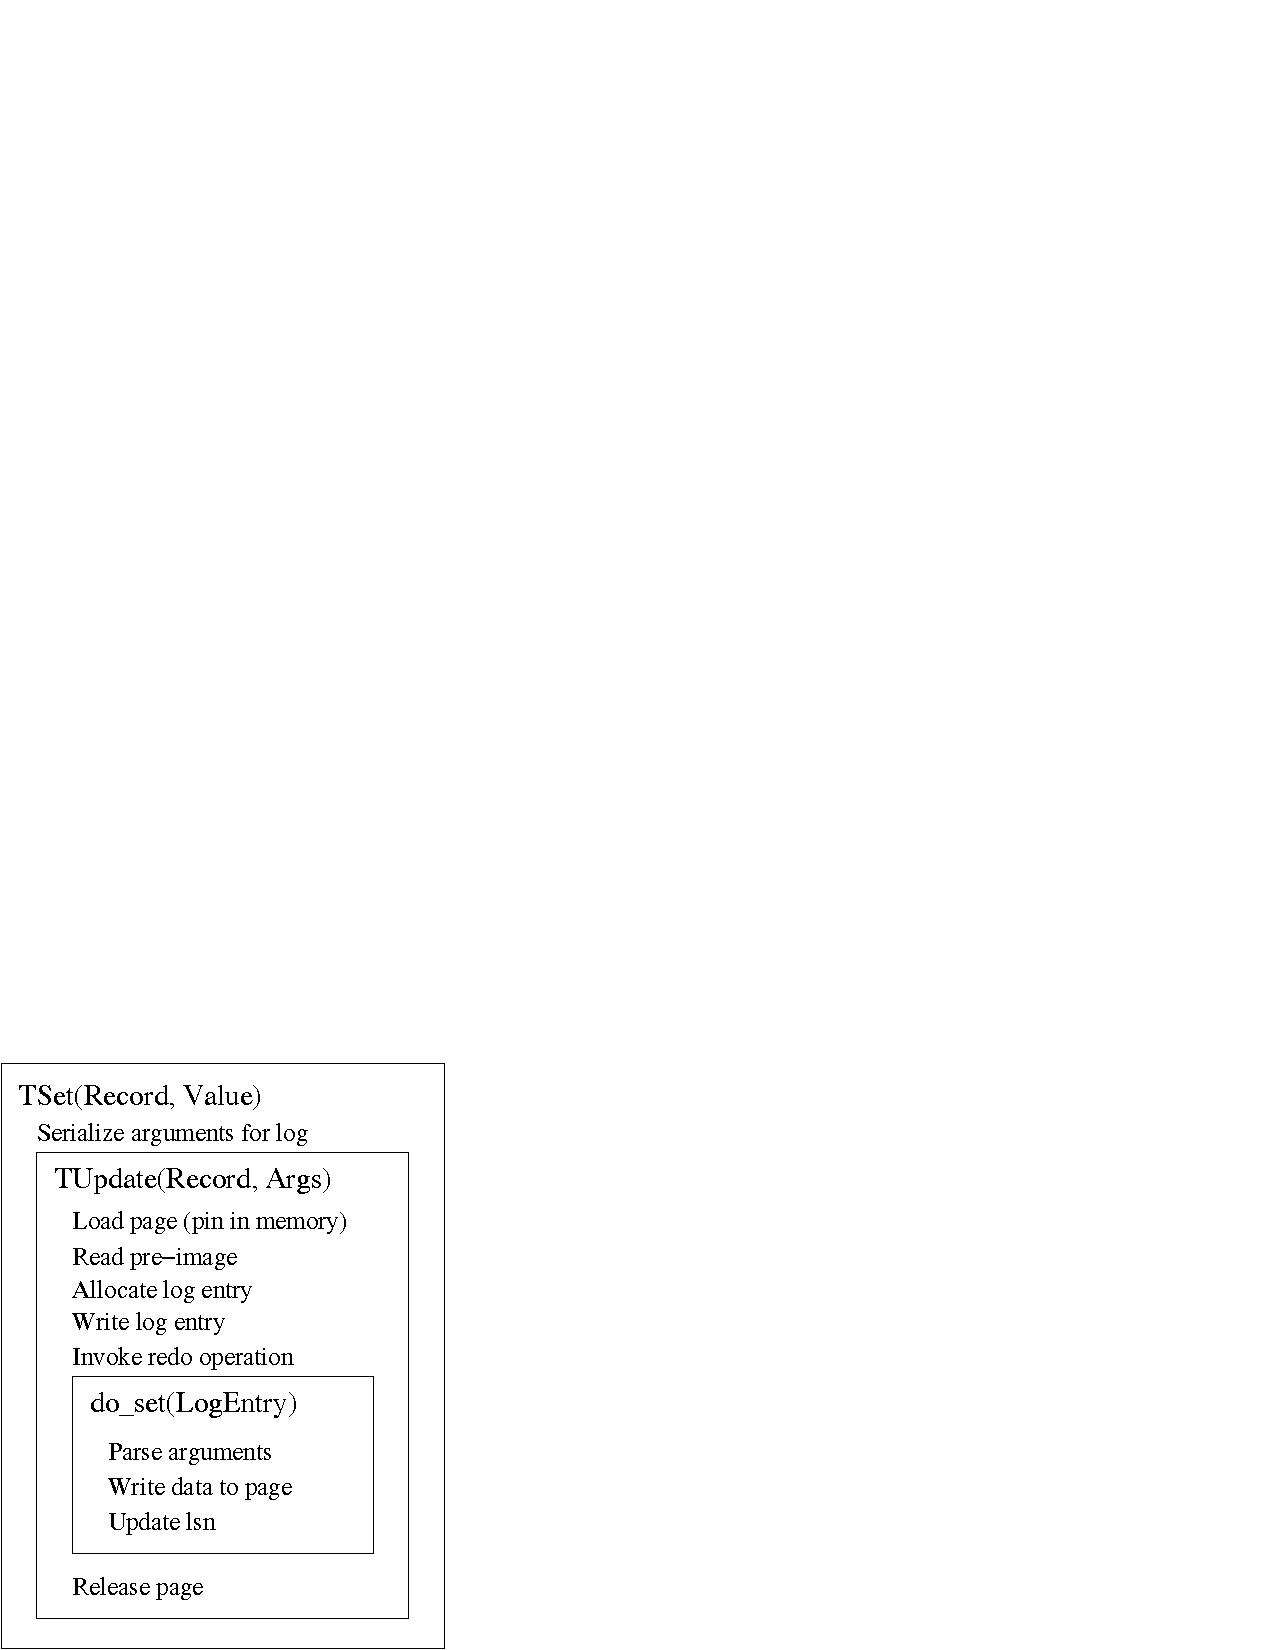
\includegraphics[%
%%  width=0.70\columnwidth]{TSetCall.pdf}
%%\end{center}
%
%\caption{\label{cap:Tset}Runtime behavior of a simple operation. Tset() and redoSet() are
%extensions that implement a new operation, while Tupdate() is built in. New operations
%need not be aware of the complexities of LLADD.}
%\end{figure}
%
%This way, the operation's behavior during recovery's redo phase (an
%uncommon case) will be identical to the behavior during normal processing,
%making it easier to spot bugs. Similarly, undo and redo operations take
%an identical set of parameters, and undo during recovery is the same 
%as undo during normal processing.  This makes recovery bugs more obvious and allows redo
%functions to be reused to implement undo. 
%
%Although any latches acquired by the wrapper function will not be
%reacquired during recovery, the redo phase of the recovery process
%is single threaded. Since latches acquired by the wrapper function
%are held while the log entry and page are updated, the ordering of
%the log entries and page updates associated with a particular latch
%will be consistent. Because undo occurs during normal operation, 
%some care must be taken to ensure that undo operations obtain the 
%proper latches.
%

%\subsection{Summary}
%
%This section presented a relatively simple set of rules and patterns
%that a developer must follow in order to implement a durable, transactional
%and highly-concurrent data structure using LLADD:

  % rcs:The last paper contained a tutorial on how to use LLADD, which 
  % should be shortend or removed from this version, so I didn't paste it 
  % in.  However, it made some points that belong in this section
  % see: ##2##

%\begin{enumerate}
  %
  % need block diagram here.  4 blocks:
  %
  % App specific:
  %
  %  - operation wrapper
  %  - operation redo fcn
  %
  % LLADD core:
  % 
  %  - logger
  %  - page file
  %
  % lock manager, etc can come later...
  %

%  \item {\bf {}``Write ahead logging protocol'' vs {}``Data structure implementation''}
%
%A LLADD operation consists of some code that manipulates data that has
%been stored in transactional pages.  These operations implement
%high-level actions that are composed into transactions.  They are
%implemented at a relatively low level, and have full access to the
%ARIES algorithm.  Applications are implemented on top of the
%interfaces provided by an application-specific set of operations.
%This allows the the application, the operation, and LLADD itself to be
%independently improved. 

\subsection{Operation Implementation}

%  \item {\bf  ARIES provides {}``transactional pages'' }

LLADD is designed to allow application developers to easily add new
data representations and data structures by defining new operations
that can be used to provide transactions.  There are a number of
constraints that these extensions must obey:

\begin{itemize}
\item Pages should only be updated inside of a redo or undo function.
\item An update to a page should update the LSN. 
\item If the data read by the wrapper function must match the state of
the page that the redo function sees, then the wrapper should latch
the relevant data.
\item Redo operations should address pages by their physical offset,
while Undo operations should use a more permanent address (such as
index key) if the data may move between pages over time.
\end{itemize}

There are multiple ways to ensure the atomicity of operations:

\begin{itemize}
\item An operation that spans pages can be made atomic by simply
wrapping it in a nested top action and obtaining appropriate latches
at runtime.  This approach reduces development of atomic page spanning
operations to something very similar to conventional multithreaded
development using mutexes for synchroniztion.  Unfortunately, this
mode of operation writes redundant undo entry to the log, and has
performance implications that will be discussed later.  However, for
most circumstances, the ease of development with nested top actions
outweighs the difficulty verifying the correctness of implementations
that use the next method.

\item It nested top actions are not used, an undo operation must
correctly update a data structure if any prefix of its corresponding
redo operations are applied to the structure, and if any number of
intervening operations are applied to the structure.  In the best
case, this simply means that the operation should fail gracefully if
the change it should undo is not already reflected in the page file.
However, if the page file must temporarily lose consistency, then the
undo operation must be aware of this, and be able to handle all cases
that could arise at recovery time.  Figure~\ref{linkedList} provides
an example of the sort of details that can arise in this case.
\end{itemize}

We believe that it is reasonable to expect application developers to
develop extensions that follow this set of constraints, but have not
confirmed this experimentally.  Furthermore, we plan to develop a
number of tools that will automatically verify or test new operation
implementations behavior with respect to these constraints, and
behavior during recovery.

Because undo and redo operations during normal operation and recovery
are similar, most bugs will be found with conventional testing
strategies.  There is some hope of verifying the atomicity property if
nested top actions are used.  Whether or not nested top actions are
implemented, randomized testing or more advanced sampling techniques
could be used to check operation behavior under various recovery
conditions and thread schedules.~\cite{OSDIFSModelChecker}

However, as we will see in Section~\ref{OASYS}, some applications may
have valid reasons to ``break'' recovery semantics.  It is unclear how
useful such testing tools will be in this case.

Note that the ARIES algorithm is extremely complex, and we have left
out most of the details needed to understand how ARIES works, or to 
implement it correctly.
Yet, we believe we have covered everything that a programmer needs
 to know in order to implement new data structures using the 
functionality that our library provides. This was possible due to the encapsulation
of the ARIES algorithm inside of LLADD, which is the feature that
most strongly differentiates LLADD from other, similar libraries.

%We hope that this will increase the availability of transactional
%data primitives to application developers.



\begin{enumerate}

  \item {\bf Log entries as a programming primitive }

  %rcs: Not quite happy with existing text; leaving this section out for now.
  %
  %  Need to make some points the old text did not make:
  %
  %     - log optimizations (for space) can be very important.  
  %           - many small writes 
  %           - large write of small diff 
  %           - app overwrites page many times per transaction (for example, database primary key)
  %    We have solutions to #1 and 2.  A general solution to #3 involves 'scrubbing' a logical log of redundant operations.
  %    
  %        - Talk about virtual async log thing...
  %           - reordering
  %           - distribution

  \item {\bf Error handling with compensations as {}``abort() for C''}

  % stylized usage of Weimer -> cheap error handling, no C compiler modifications...

  \item {\bf Concurrency models are fundamentally application specific, but
  record/page level locking and index locks are often a nice trade-off}  @todo We sort of cover this above

%  \item {\bf {}``latching'' vs {}``locking'' - data structures internal to
%  LLADD are protected by LLADD, allowing applications to reason in
%  terms of logical data addresses, not physical representation. Since
%  the application may define a custom representation, this seems to be
%  a reasonable tradeoff between application complexity and
%  performance.}
%
%  \item {\bf Non-interleaved transactions vs. Nested top actions
%  vs. Well-ordered writes.}

    % key point: locking + nested top action = 'normal' multithreaded
    %software development! (modulo 'obvious' mistakes like algorithmic
    %errors in data structures, errors in the log format, etc)
    
    % second point: more difficult techniques can be used to optimize
    % log bandwidth. _in ways that other techniques cannot provide_ 
    % to application developers.



\end{enumerate}

\section{Sample operations}

\begin{enumerate}

  \item {\bf Atomic file-based transactions. 
    
    Prototype blob implementation  using force, shadow copies (it is trivial to implement given transactional
  pages).  

  File systems that implement atomic operations may allow
  data to be stored durably without calling flush() on the data
  file. 

  Current implementation useful for blobs that are typically
  changed entirely from update to update, but smarter implementations
  are certainly possible. 

  The blob implementation primarily consists
  of special log operations that cause file system calls to be made at
  appropriate times, and is simple, so it could easily be replaced by
  an application that frequently update small ranges within blobs, for
  example.}

  \item {\bf Index implementation - modular hash table. Relies on separate
  linked list, expandable array implementations.}

\subsection{Array List}
   % Example of how to avoid nested top actions
\subsection{Linked Lists}
   % Example of two different page allocation strategies.
   % Explain how to implement linked lists w/out NTA's (even though we didn't do that)?

\subsection{Linear Hash Table\label{sub:Linear-Hash-Table}}
   % The implementation has changed too much to directly reuse old section, other than description of linear hash tables:

Linear hash tables are hash tables that are able to extend their bucket
list incrementally at runtime. They work as follows. Imagine that
we want to double the size of a hash table of size $2^{n}$, and that
the hash table has been constructed with some hash function $h_{n}(x)=h(x)\, mod\,2^{n}$.
Choose $h_{n+1}(x)=h(x)\, mod\,2^{n+1}$ as the hash function for
the new table. Conceptually we are simply prepending a random bit
to the old value of the hash function, so all lower order bits remain
the same. At this point, we could simply block all concurrent access
and iterate over the entire hash table, reinserting values according
to the new hash function. 

However, because of the way we chose $h_{n+1}(x),$ we know that the
contents of each bucket, $m$, will be split between bucket $m$ and
bucket $m+2^{n}$. Therefore, if we keep track of the last bucket that
was split, we can split a few buckets at a time, resizing the hash
table without introducing long pauses while we reorganize the hash
table~\cite{lht}. We can handle overflow using standard techniques;
LLADD's linear hash table simply uses the linked list implementations
described above.  The bucket list is implemented by reusing the array
list implementation described above.

% Implementation simple!  Just slap together the stuff from the prior two sections, and add a header + bucket locking.

  \item {\bf Asynchronous log implementation/Fast
  writes. Prioritization of log writes (one {}``log'' per page)
  implies worst case performance (write, then immediate read) will
  behave on par with normal implementation, but writes to portions of
  the database that are not actively read should only increase system
  load (and not directly increase latency)} This probably won't go
  into the paper.  As long as the buffer pool isn't thrashing, this is
  not much better than upping the log buffer.

  \item {\bf Custom locking. Hash table can support all of the SQL
  degrees of transactional consistency, but can also make use of
  application-specific invariants and synchronization to accommodate
  deadlock-avoidance, which is the model most naturally supported by C
  and other programming languages.}  This is covered above, but we
  might want to mention that we have a generic lock manager
  implemenation that operation implementors can reuse.  The argument
  would be stronger if it were a generic hierarchical lock manager.

%Many plausible lock managers, can do any one you want.
%too much implemented part of DB; need more 'flexible' substrate.

\end{enumerate}

\section{Benchmarks}

\subsection{Conventional workloads}

Existing database servers and transactional libraries are tuned to
support OLTP (Online Transaction Processing) workloads well.  Roughly
speaking, the workload of these systems is dominated by short
transactions and response time is important.  We are confident that a
sophisticated system based upon our approach to transactional storage
will compete well in this area, as our algorithm is based upon ARIES,
which is the foundation of IBM's DB/2 database.  However, our current
implementation is geared toward simpler, specialized applications, so
we cannot verify this directly.  Instead, we present a number of
microbenchmarks that compare our system against Berkeley DB, the most
popular transactional library.  Berkeley DB is a mature product and is
actively maintained.  While it currently provides more functionality
than our current implementation, we believe that our architecture
could support a broader range of features than provided by BerkeleyDB,
which is a monolithic system.

The first test measures the throughput of a single long running
transaction that generates an loads a synthetic data set into the
library.  For comparison, we provide throughput for many different
LLADD operations, and BerkeleyDB's DB\_HASH hashtable implementation,
and lower level DB\_RECNO record number based interface.

@todo fill in numbers here.

The second test measures the two library's ability to exploit
concurrent transactions to reduce logging overhead.  Both systems
implement a simple optimization that allows multiple calls to commit()
to be serviced by a single synchronous disk request.  

@todo analysis

The final test measures the maximum number of sustainable transactions
per second for the two libraries.  In these cases, we generate a
uniform number of transactions per second by spawning a fixed nuber of
threads, and varying the number of requests each thread issues per
second, and report the cumulative density of the distribution of
response times for each case.

@todo analysis / come up with a more sane graph format.

\subsection{Object Serialization}\label{OASYS}

Object serialization performance is extremely important in modern web
service systems such as EJB.  Object serialization is also a
convenient way of adding persistant storage to an existing application
without developing an explicit file format or dealing with low level
I/O interfaces.

A simple object serialization scheme would bulk-write and bulk-read
sets of application objects to an operating system file.  These
schemes suffer from high read and write latency, and do not handle
small updates well.  More sophisticated schemes store each object in a
seperate randomly accessible record, such as a database tuple, or
Berkeley DB hashtable entry.  These schemes allow for fast single
object reads and writes, and are typically the solutions used by
application services.

Unfortunately, most of these schemes ``double buffer'' application
data.  Typically, the application maintains a set of in-memory objects
which may be accessed with low latency.  The backing data store
maintains a seperate buffer pool which contains serialized versions of
the objects in memory, and corresponds to the on-disk representation
of the data.  Accesses to objects that are only present in the buffer
pool incur ``medium latency,'' as they must be deserialized before the
application may access them.  Finally, some objects may only reside on
disk, and may only be accessed with high latency.

Since these applications are typically data-centric, it is important
to make efficient use of system memory in order to reduce hardware
costs.  A straightforward solution to this problem would be to bound
the amount of memory the application may consume by preventing it from
caching deserialized objects.  This scheme conserves memory, but it
incurs the cost of an in-memory deserialization to read the object,
and an in-memory deserialization/serialization cycle to write to an
object.

Alternatively, the amount of memory consumed by the buffer pool could
be bounded to some small value, and the application could maintain a
large object cache.  This scheme would incur no overhead for a read
request.  However, it would incur the overhead of a disk-based
serialization in order to service a write request.\footnote{In
practice, the transactional backing store would probably fetch the
page that contains the object from disk, causing two disk I/O's to be
issued.}

LLADD's architecture allows us to apply two interesting optimizations
to such object serialization schemes.  First, since LLADD supports
custom log entries, it is trivial to have it store diffs of objcts to
the log instead of writing the entire object to log during an update.
Such an optimization would be difficult to achieve with Berkeley DB,
but could be performed by a database server if the fields of the
objects were broken into database table columns.  It is unclear if
this optimization would outweigh the overheads associated with an SQL
based interface.

% @todo WRITE SQL OASYS BENCHMARK!!

The second optimization is a bit more sophisticated, but still easy to
implement in LLADD.  We do not believe that it would be possible to
achieve using existing relational database systems, or with Berkeley
DB.  

LLADD services a request to write to a record by pinning (and possibly
reading in) a page, generating a log entry, writing the
new record value to the page, and unpinning the page.

If LLADD knows that the client will not ask to read the record, then
there is no real reason to update the version of the record in the
page file.  In fact, if no undo or redo information needs to be
generated, there is no need to bring the page into memory at all.
There are two scenarios that allow LLADD to avoid loading the page:

First, the application may not be interested in transaction atomicity.
In this case, by writing no-op undo information instead of real undo
log entries, LLADD could guarantee that some prefix of the log will be
applied to the page file after recovery.  The redo information is
already available; the object is in the application's cache.
``Transactions'' could still be durable, as commit() could be used to
force the log to disk.

Second, the application could provide the undo information to LLADD.
This could be implemented in a straightforward manner by adding
special accessor methods to the object which generate undo information
as the object is updated in memory.  For our benchmarks, we opted for
the first approach.

We have removed the need to use the on-disk version of the object to
generate log entries, but still need to guarantee that the application
will not attempt to read a stale record from the page file.  This
problem also has a simple solution.  In order to service a write
request made by the application, the cache calls a special
``update()'' operation.  This method only writes a log entry.  If the
cache must evict an object from cache, it performs a special ``flush()''
operation.  This method writes the object to the buffer pool (and
probably incurs the cost of disk I/O), using a LSN recorded by the
most recent update() call that was associated with the object.  Since
LLADD implements no-force, it does not matter to recovery if the
version of the object in the page file is stale.

An observant reader may have noticed a subtle problem with this
scheme.  More than one object may reside on a page, and we do not
constrain the order in which the cache calls flush() to evict objects.
Recall that the version of the LSN on the page implies that all
updates {\em up to} and including the page LSN have been applied.
Nothing stops our current scheme from breaking this invariant.  

We have two potential solutions to this problem.  One solution is to
implement a cache eviction policy that respects the ordering of object
updates on a per-page basis and could be implemented using one or
more priority queues.  Instead of interfering with the eviction policy
of the cache (and keeping with the theme of this paper), we sought a
solution that leverages LLADD's interfaces instead.

We can force LLADD to ignore page LSN values when considering our
special update() log entries during the REDO phase of recovery.  This
forces LLADD to re-apply the diffs in the same order the application
generated them in.  This works as intended because we use an
idempotent diff format that will produce the correct result even if we
start with a copy of the object that is newer than the first diff that
we apply.

The only remaining detail is to implement a custom checkpointing
algorithm that understands the page cache.  In order to produce a
fuzzy checkpoint, we simply iterate over the object pool, calculating
the minimum lsn of the objects in the pool.\footnote{This LSN is distinct from
the one used by flush(); it is the lsn of the object's {\em first}
call to update() after the object was added to the cache.}  At this
point, we can invoke a normal ARIES checkpoint with the restriction
that the log is not truncated past the minimum LSN encountered in the
object pool.\footnote{Because LLADD does not yet implement
checkpointing, we have not implemented this checkpointing scheme.}

We implemented a LLADD plugin for OASYS, a C++ object serialization
library includes various object serialization backends, including one
for Berkeley DB.  The LLADD plugin makes use of the optimizations
described in this section, and was used to generate Figure~[TODO].
For comparison, we also implemented a non-optimized LLADD plugin to
factor out performance and implementation differences between LLADD
and Berkeley DB.

Initially, OASYS did not support an object cache, so this
functionality was added.  Berkeley DB and LLADD's variants were run
using identical cache settings and random seeds for load generation.
Even though the serialization requests were serviced out of operating
system cache, we see that the optimized LLADD implemenation has a
clear advantage under most circumstances, suggesting that the overhead
incurred by generating diffs and having seperate update() and flush()
calls is negligible compared to the savings in log bandwidth and
buffer pool overhead that the optimizations provide.

Ignoring the checkpointing scheme and a small change needed in the
recovery algorithm, the operations required for these two
optimizations are roughly 150 lines of C code, including whitespace,
comments and boilerplate function registrations.  While the reasoning
required to ensure the correctness of this code was complex, the
simplicity of the implementation is encouraging.

@todo analyse OASYS data.

\subsection{Transitive closure}

@todo implement transitive closu....

%\begin{enumerate}
%
%  \item {\bf Comparison of transactional primatives (best case for each operator)}
%
%  \item {\bf Serialization Benchmarks (Abstract log) }
%
%    {\bf Need to define application semantics workload (write heavy w/ periodic checkpoint?) that allows for optimization.}
%    
%    {\bf All of these graphs need X axis dimensions.  Number of (read/write?) threads, maybe?}
% 
%    {\bf Graph 1:  Peak write throughput. Abstract log wins (no disk i/o, basically, measure contention on ringbuffer, and compare to log I/O + hash table insertions.)}
%
%    {\bf Graph 2:  Measure maximum average write throughput: Write throughput vs. rate of log growth.  Spool abstract log to disk.
%              Reads starve, or read stale data. }
%
%    {\bf Graph 3:  Latency @ peak steady state write throughput.  Abstract log size remains constant.  Measure read latency vs.
%               queue length.  This will show the system's 'second-order' ability to absorb spikes. }
%
%  \item {\bf Graph traversal benchmarks:  Bulk load + hot and cold transitive closure queries}
%
%  \item {\bf Hierarchical Locking - Proof of concept}
%
%  \item {\bf TPC-C (Flexibility) - Proof of concept}
%    
%   % Abstract syntax tree implementation?
%
%  \item {\bf Sample Application. (Don't know what yet?) }
%
%\end{enumerate}

\section{Future work}
\begin{enumerate}
  \item {\bf PL / Testing stuff}
  \item {\bf Explore async log capabilities further}
  \item {\bf ... from old paper}
\end{enumerate}
\section{Conclusion}


\begin{thebibliography}{99}

\bibitem[1]{multipleGenericLocking} Agrawal, et al. {\em Concurrency Control Performance Modeling: Alternatives and Implications}. TODS 12(4): (1987) 609-654

\bibitem[2]{bdb} Berkeley~DB, {\tt http://www.sleepycat.com/}

\bibitem[3]{capriccio} R. von Behren, J Condit, F. Zhou, G. Necula, and E. Brewer. {\em Capriccio: Scalable Threads for Internet Services} SOSP 19 (2003).

\bibitem[4]{relational} E. F. Codd, {\em A Relational Model of Data for Large Shared Data Banks.} CACM 13(6) p. 377-387 (1970)

\bibitem[5]{lru2s} Envangelos P. Markatos. {\em On Caching Search Engine Results}.  Institute of Computer Science, Foundation for Research \& Technology - Hellas (FORTH) Technical Report 241 (1999)

\bibitem[6]{semantic} David K. Gifford, P. Jouvelot, Mark A. Sheldon, and Jr. James W. O'Toole. {\em Semantic file systems}. Proceedings of the Thirteenth ACM Symposium on Operating Systems Principles, (1991) p. 16-25.

\bibitem[7]{physiological} Gray, J. and Reuter, A. {\em Transaction Processing: Concepts and Techniques}. Morgan Kaufmann (1993) San Mateo, CA

\bibitem[8]{hierarcicalLocking} Jim Gray, Raymond A. Lorie, and Gianfranco R. Putzulo. {\em Granularity of locks and degrees of consistency in a shared database}. In 1st International Conference on VLDB, pages 428--431, September 1975. Reprinted in Readings in Database Systems, 3rd edition.

\bibitem[9]{haerder} Haerder \& Reuter {\em "Principles of Transaction-Oriented Database Recovery." } Computing Surveys 15(4) p 287-317 (1983)

\bibitem[10]{lamb} Lamb, et al., {\em The ObjectStore System.} CACM 34(10) (1991) p. 50-63

\bibitem[11]{blink} Lehman \& Yao, {\em Efficient Locking for Concurrent Operations in B-trees.} TODS 6(4) (1981) p. 650-670

\bibitem[12]{lht} Litwin, W., {\em Linear Hashing: A New Tool for File and Table Addressing}. Proc. 6th VLDB, Montreal, Canada, (Oct. 1980) p. 212-223

\bibitem[13]{aries} Mohan, et al., {\em ARIES: A Transaction Recovery Method Supporting Fine-Granularity Locking and Partial Rollbacks Using Write-Ahead Logging.} TODS 17(1) (1992) p. 94-162

\bibitem[14]{twopc} Mohan, Lindsay \& Obermarck, {\em Transaction Management in the R* Distributed Database Management System} TODS 11(4) (1986) p. 378-396

\bibitem[15]{ariesim} Mohan, Levine. {\em ARIES/IM: an efficient and high concurrency index management method using write-ahead logging} International Converence on Management of Data, SIGMOD (1992) p. 371-380

\bibitem[16]{mysql} {\em MySQL}, {\tt http://www.mysql.com/ }

\bibitem[17]{reiser} Reiser,~Hans~T. {\em ReiserFS 4} {\tt http://www.namesys.com/ } (2004)
%
\bibitem[18]{berkeleyDB} M. Seltzer, M. Olsen. {\em LIBTP: Portable, Modular Transactions for UNIX}. Proceedings of the 1992 Winter Usenix (1992)

\bibitem[19]{lrvm} Satyanarayanan, M., Mashburn, H. H., Kumar, P., Steere, D. C., AND Kistler, J. J. {\em Lightweight Recoverable Virtual Memory}. ACM Transactions on Computer Systems 12, 1 (Februrary 1994) p. 33-57. Corrigendum: May 1994, Vol. 12, No. 2, pp. 165-172.

\bibitem[20]{newTypes} Stonebraker. {\em Inclusion of New Types in Relational Data Base } ICDE (1986) p. 262-269

%\bibitem[SLOCCount]{sloccount} SLOCCount, {\tt http://www.dwheeler.com/sloccount/ }
%
%\bibitem[lcov]{lcov} The~LTP~gcov~extension, {\tt http://ltp.sourceforge.net/coverage/lcov.php }
%


%\bibitem[Beazley]{beazley} D.~M.~Beazley and P.~S.~Lomdahl, 
%{\em Message-Passing Multi-Cell Molecular Dynamics on the Connection
%Machine 5}, Parall.~Comp.~ 20 (1994) p. 173-195.
%
%\bibitem[RealName]{CitePetName} A.~N.~Author and A.~N.~Other, 
%{\em Title of Riveting Article}, JournalName VolNum (Year) p. Start-End
%
%\bibitem[ET]{embed} Embedded Tk, \\
%{\tt ftp://ftp.vnet.net/pub/users/drh/ET.html}
%
%\bibitem[Expect]{expect} Don Libes, {\em Exploring Expect}, O'Reilly \& Associates, Inc. (1995).
%
%\bibitem[Heidrich]{heidrich} Wolfgang Heidrich and Philipp Slusallek, {\em
%Automatic Generation of Tcl Bindings for C and C++ Libraries.},
%USENIX 3rd Annual Tcl/Tk Workshop (1995).
%
%\bibitem[Ousterhout]{ousterhout} John K. Ousterhout, {\em Tcl and the Tk Toolkit}, Addison-Wesley Publishers (1994).
%
%\bibitem[Perl5]{perl5} Perl5 Programmers reference,\\
%{\tt http://www.metronet.com/perlinfo/doc}, (1996).
%
%\bibitem[Wetherall]{otcl} D. Wetherall, C. J. Lindblad, ``Extending Tcl for
%Dynamic Object-Oriented Programming'', Proceedings of the USENIX 3rd Annual Tcl/Tk Workshop (1995).

\end{thebibliography}



\end{document}
